\section{Dissimilarity Constraint} \label{sec:dissimilarityconstraint}

\input{fig/dissimilarity_statistic.tex}

To compute this statistic, we randomly sampled 5000 target tags.
Then, for each target tag we randomly sampled tags until we found a secondarily-sampled tag that was within a 0.01 match distance radius of the target and a secondarily-sampled tag that was outside a 0.99 match distance radius of the target.
Finally, we computed the match distance between the pair of secondarily-sampled tags.
Figure \ref{fig:dissimilarity_statistic} summarizes this process.

\begin{figure}[!htbp]

\begin{center}
\begin{subfigure}[b]{\linewidth}
\begin{minipage}{0.5\linewidth}

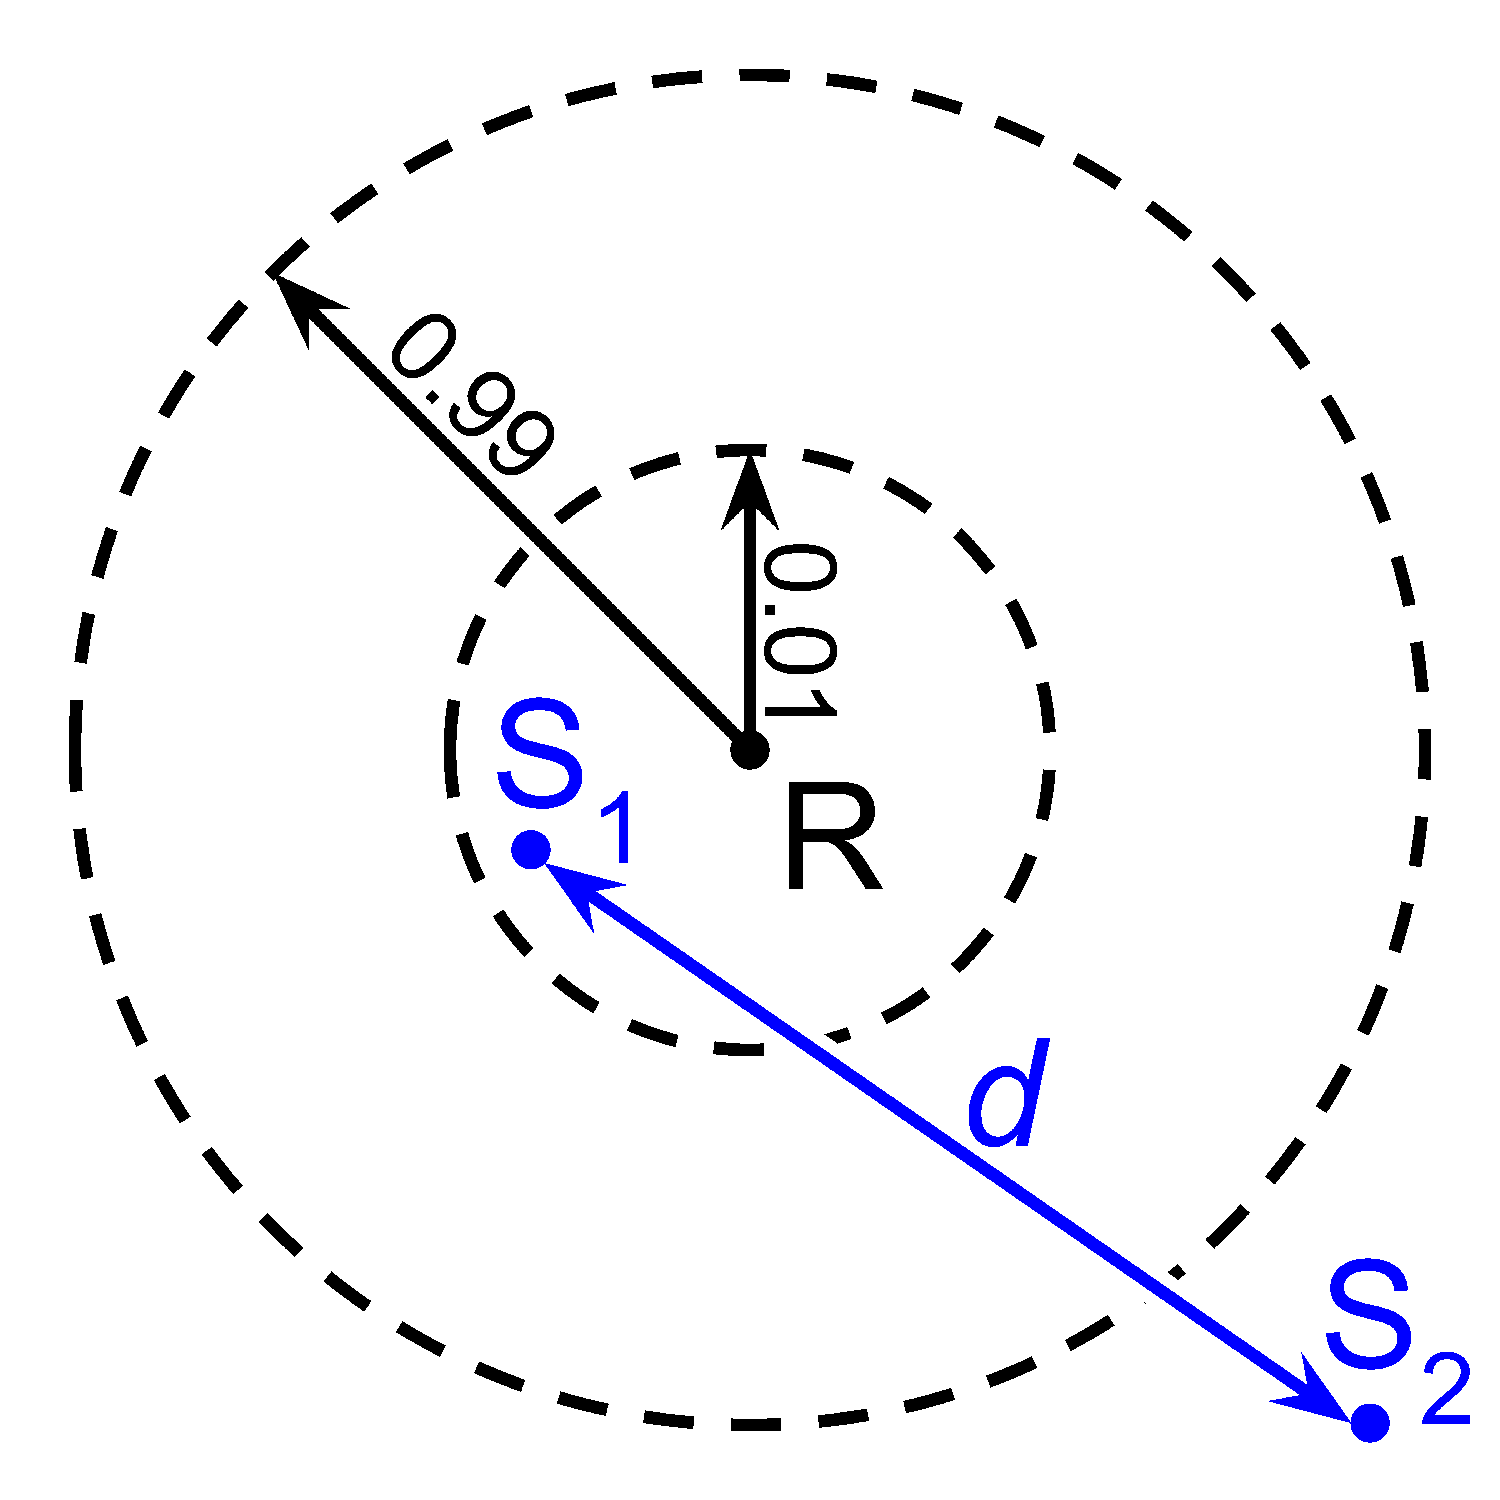
\includegraphics[width=0.75\linewidth]{img/elasticity-statistic}

\end{minipage}
\begin{minipage}{0.5\linewidth}
\caption{
Sampling process used to measure dissimilarity constraint.
First, a target tag $R$ was randomly sampled.
Then, tags were randomly drawn until a tag $S_1$ with distance to $R$ less than 0.01 was obtained.
Next, tags were randomly drawn until a tag $S_1$ with distance to $R$ more than 0.99 was obtained.
Finally, dissimilarity constraint was measured as the distance $d$ between $S_1$ and $S_2$.
}
\label{fig:dissimilarity_statistic}
\end{minipage}

\end{subfigure}

\begin{subfigure}[b]{\linewidth}
\begin{minipage}{0.6\linewidth}
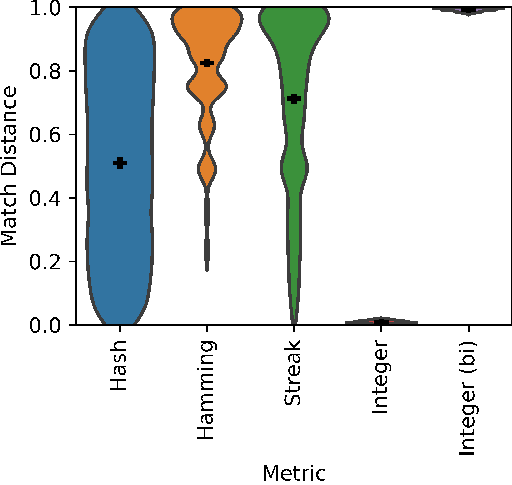
\includegraphics[width=\linewidth]{img/sphere_reverse/bitweight=0dot5+seed=1+title=dimensionality_violinplot+_data_hathash_hash=93f97a11cb443d35+_script_fullcat_hash=d1692569f79e33f8+ext=}
\end{minipage}
\begin{minipage}{0.35\linewidth}
\caption{
Mean dissimilarity constraint values for each metric.
Horizontal ticks represent means.
Error bars represent 95\% confidence intervals.
Violin plots show kernel density estimates for distribution of dissimilarity constrant.
}
\label{fig:sphere_reverse_distnplot}
\end{minipage}
\end{subfigure}
\begin{subfigure}[b]{\columnwidth}
\centering
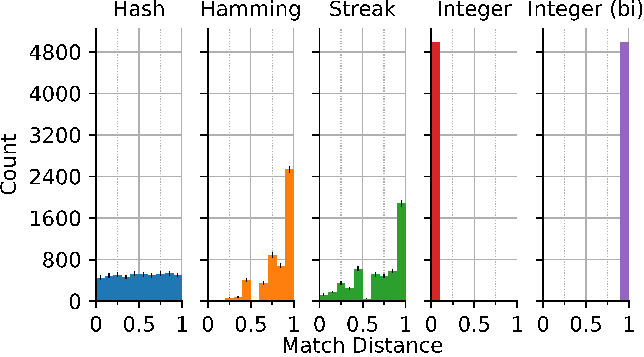
\includegraphics[width=\columnwidth]{img/sphere_reverse/bitweight=0dot5+seed=1+title=dimensionality_distnplot+viz=hist+_data_hathash_hash=93f97a11cb443d35+_script_fullcat_hash=cda229fb13f5a152+ext=}
\caption{
Frequency of sampled dissimilarity constraint values in each match distance decile.
Error bars are 95\% confidence intervals calculated using the Wilson score method with continuity correction \citep{newcombe1998two}.
}
\label{fig:sphere_reverse_barplot}
\end{subfigure}

\caption{
Dissimilarity constraint of tag-matching metrics.
Figure \ref{fig:dissimilarity_statistic} summarizes the sampling process used to measure similarity constraint.
Figures \ref{fig:sphere_reverse_barplot} and \ref{fig:sphere_reverse_distnplot} compare distributions of similarity constraint across metrics.
Supplementary Figure \ref{fig:sphere_reverse_supp} visualizes the cumulative distribution of all sampled dissimilarity constraint values for each metric.
}
\label{fig:sphere_reverse}

\end{center}
\end{figure}


Supplementary Figure \ref{fig:sphere_barplot} provides our estimate of the dissimilarity constraint statistic for each metric, with error bars representing a 95\% confidence interval.
Supplementary Figure \ref{fig:sphere_distnplot} shows the distribution of the dissimilarity constraint statistic values among the 5000 replicate samples in greater detail.

These results tell a story across metrics very to the simiarity constraint results.
The hash metric exhibited no geometric structure.
The streak metric exhibited some geometric structure in the mean case (mean secondarily-sampled distance 0.7127), but outcomes that strongly broke geometric constraints were also observed (we observed distances between secondarily-sampled tags as low as 0.0002).
The hamming metric exhibited stronger geometric structure in the mean case (mean secondarily-sampled distance 0.8248) and had less extreme tail-end outcomes (we observed match distances between the secondarily-sampled tags only as low as 0.2355).
The bidirectional integer metric was highly constrained in both the mean and tail-end cases.
The smallest distance between secondarily-sampled tags was 0.9802.
Again, the unidirectional integer metric exhibited a quirky result due to its noncommutative nature.
The mean distance between secondarily-sampled tags was 0.0100.
As shown in Figure \ref{fig:sphere_distnplot}, all secondarily-sampled distances oberved with this metric were extremely small.
Under this metric, if you sample a tag that is close to a target it will be numerically slightly larger than the target.
Likewise, if you sample a tag that is very far from a target, it will be numerically slightly smaller than the target (due to wraparound).
Then, explaining this counterintuitive result, the distance from the slightly smaller to the larger tag will be small.
